\chapter{Constants, functions, and variables}
\label{chap:let}
%
In the previous chapter, we saw how to use F\# as a calculator working with literals, operators and built-in functions. To save time and make programs easier to read and debug, it is useful to bind expressions to identifiers either as new constants, functions or operators. For example, to solve for  $x$, when
\begin{equation}
  a x^2+bx+c = 0
\end{equation}
we use the quadratic formula from elementary algebra,
\begin{equation}
  x = \frac{-b\pm\sqrt{b^2-4ac}}{2a},
\end{equation}
and write a small program that defines functions calculating relevant values for any set of coefficients,
%
\fs{identifiersExample}{Finding roots for quadratic equations using function name binding.}
%
Here 3 functions are defined as \lstinline!determinant!, \lstinline!postiveSolution!, and \lstinline!negativeSolution! are defined, and applied to 3 values named \lstinline!a!, \lstinline!b!, and \lstinline!c!, and the results are named \lstinline!d!, \lstinline!xn!, and \lstinline!xp!. These names are examples of identifiers, and with these, we may reuse the quadratic formulas and calculated values later, while avoiding possible typing mistakes and reducing amount of code, which needs to be debugged.

Before we begin a deeper discussion note that F\# has adheres to two different syntax, regular and \idx[lightweight syntax]{ligthweight}. In the regular syntax, newlines and whitespaces are generally ignored, while in lightweight syntax, certain keywords and lexemes may be replaced by specific use of newlines and whitespaces. Lightweight syntax is the most common, but the syntaxes may be mixed, and we will highlight the options, when relevant.

The use of identifiers is central in programming. For F\# not to be confused by built-in functionality, identifiers must follow a specific grammar: An identifier must start with a letter, but can be followed by zero or more of letters, digits, and a range of special characters except SP, LF, and CR (space, line feed, and carriage return). An identifier must not be a keyword or a reserved-keyword listed in Figures~\ref{fig:keywords}, \ref{fig:reservedKeywords}, \ref{fig:symbolicKeywords}, and \ref{fig:reservedSymbolicKeywords}
\begin{figure}
  \mbox{\lstinline{abstract},} \mbox{\lstinline{and},} \mbox{\lstinline{as},} \mbox{\lstinline{assert},} \mbox{\lstinline{base},} \mbox{\lstinline{begin},} \mbox{\lstinline{class},} \mbox{\lstinline{default},} \mbox{\lstinline{delegate},} \mbox{\lstinline{do},} \mbox{\lstinline{done},} \mbox{\lstinline{downcast},} \mbox{\lstinline{downto},} \mbox{\lstinline{elif},} \mbox{\lstinline{else},} \mbox{\lstinline{end},} \mbox{\lstinline{exception},} \mbox{\lstinline{extern},} \mbox{\lstinline{false},} \mbox{\lstinline{finally},} \mbox{\lstinline{for},} \mbox{\lstinline{fun},} \mbox{\lstinline{function},} \mbox{\lstinline{global},} \mbox{\lstinline{if},} \mbox{\lstinline{in},} \mbox{\lstinline{inherit},} \mbox{\lstinline{inline},} \mbox{\lstinline{interface},} \mbox{\lstinline{internal},} \mbox{\lstinline{lazy},} \mbox{\lstinline{let},} \mbox{\lstinline{match},} \mbox{\lstinline{member},} \mbox{\lstinline{module},} \mbox{\lstinline{mutable},} \mbox{\lstinline{namespace},} \mbox{\lstinline{new},} \mbox{\lstinline{null},} \mbox{\lstinline{of},} \mbox{\lstinline{open},} \mbox{\lstinline{or},} \mbox{\lstinline{override},} \mbox{\lstinline{private},} \mbox{\lstinline{public},} \mbox{\lstinline{rec},} \mbox{\lstinline{return},} \mbox{\lstinline{sig},} \mbox{\lstinline{static},} \mbox{\lstinline{struct},} \mbox{\lstinline{then},} \mbox{\lstinline{to},} \mbox{\lstinline{true},} \mbox{\lstinline{try},} \mbox{\lstinline{type},} \mbox{\lstinline{upcast},} \mbox{\lstinline{use},} \mbox{\lstinline{val},} \mbox{\lstinline{void},} \mbox{\lstinline{when},} \mbox{\lstinline{while},} \mbox{\lstinline{with},} and \mbox{\lstinline{yield}.}
  \caption{List of keywords in F\#.}
  \label{fig:keywords}
\end{figure}
\begin{figure}
  \mbox{\lstinline{atomic},} \mbox{\lstinline{break},} \mbox{\lstinline{checked},} \mbox{\lstinline{component},} \mbox{\lstinline{const},} \mbox{\lstinline{constraint},} \mbox{\lstinline{constructor},} \mbox{\lstinline{continue},} \mbox{\lstinline{eager},} \mbox{\lstinline{fixed},} \mbox{\lstinline{fori},} \mbox{\lstinline{functor},} \mbox{\lstinline{include},} \mbox{\lstinline{measure},} \mbox{\lstinline{method},} \mbox{\lstinline{mixin},} \mbox{\lstinline{object},} \mbox{\lstinline{parallel},} \mbox{\lstinline{params},} \mbox{\lstinline{process},} \mbox{\lstinline{protected},} \mbox{\lstinline{pure},} \mbox{\lstinline{recursive},} \mbox{\lstinline{sealed},} \mbox{\lstinline{tailcall},} \mbox{\lstinline{trait},} \mbox{\lstinline{virtual},} and \mbox{\lstinline{volatile}.}
  \caption{List of reserved keywords for possible future use in F\#.}
  \label{fig:reservedKeywords}
\end{figure} 
\begin{figure}
  \mbox{\lstinline{let!},} \mbox{\lstinline{use!},} \mbox{\lstinline{do!},} \mbox{\lstinline{yield!},} \mbox{\lstinline{return!},} \mbox{\lstinline{|},} \mbox{\lstinline{->},} \mbox{\lstinline{<-},} \mbox{\lstinline{.},} \mbox{\lstinline{:},} \mbox{\lstinline{(},} \mbox{\lstinline{)},} \mbox{\lstinline{[},} \mbox{\lstinline{]},} \mbox{\lstinline{[<},} \mbox{\lstinline{>]},} \mbox{\lstinline{[|},} \mbox{\lstinline{|]},} \mbox{\lstinline{\{},} \mbox{\lstinline{\}},} \mbox{\lstinline{'},} \mbox{\lstinline{#},} \mbox{\lstinline{:?>},} \mbox{\lstinline{:?},} \mbox{\lstinline{:>},} \mbox{\lstinline{..},} \mbox{\lstinline{::},} \mbox{\lstinline{:=},} \mbox{\lstinline{;;},} \mbox{\lstinline{;},} \mbox{\lstinline{=},} \mbox{\lstinline{_},} \mbox{\lstinline{?},} \mbox{\lstinline{??},} \mbox{\lstinline{(*)},} \mbox{\lstinline{<@},} \mbox{\lstinline{@>},} \mbox{\lstinline{<@@},} and \mbox{\lstinline{@@>}.} 
  \caption{List of symbolic keywords in F\#.}
  \label{fig:symbolicKeywords}
\end{figure}
\begin{figure}
  \mbox{\lstinline{\~}} and \mbox{\lstinline{`}}.
  \caption{List of reserved symbolic keywords for possible future use F\#.}
  \label{fig:reservedSymbolicKeywords}
\end{figure}

For characters in the Basic Latin Block, i.e., the first 128 code points alias ASCII characters, an ident is,
%
\begin{lstlisting}[language=ebnf]
dDigit = "0" | "1" | "2" | "3" | "4" | "5" | "6" | "7" | "8" | "9"
letter = "A" | "B" | ... |  "Z" | "a" | "b" | ... | "z"
specialChar = "_"
ident = (letter | "_") {letter | dDigit | specialChar}
\end{lstlisting}
%
Thus, examples of identifiers are \lstinline{a}, \lstinline{theCharacter9}, \lstinline{Next_Word}, \lstinline{_tok}. The for the full definition, \lstinline[language=ebnf]{letter = Lu | Ll | Lt | Lm | Lo | Nl} and \lstinline[language=ebnf]{specialChar = Pc | Mn | Mc | Cf}, which referes to the Unicode general categories described in Appendix~\ref{sec:unicode}, and there are currently 19.345 possible Unicode code points in the \lstinline[language=ebnf]{letter} category and 2.245 possible Unicode code points in the \lstinline[language=ebnf]{specialChar} category. 
Binding expressions to identifiers is done with the keyword \keyword{let}, using the following simplified syntax:
%
\begin{lstlisting}[language=ebnf]
arg = ident | "(" ident ":" type ")"
argList = arg | arg argList
identOrOp = ident | ( operatorName )
valueDefn = ["mutable "] ident  [":" type] "=" expr
functionDefn = ident-or-op argList [":" type] "=" expr "
expr = ... 
  | "let" valueDefn "in" expr  (* binding a value or variable *)
  | "let" functionDefn "in" expr (* binding a function or operator *)
  | "fun" argList "->" expr (* a function as value *)
  | expr ":" type (* type annotation *)
  | "begin" expr "end" (* alternative block expression *)
  | expr; expr (* sequence of expression *)
  | ...
\end{lstlisting}
which will be discussed in the following.\jon{Spec-4.0 Section 6.6, function-or-value-defns, possible Mono deviation from specification: let rec functionDefn and functionDefn requires newline before and.}

\section{Values}
Binding identifiers to literals or expressions that are evaluated to be values is called value binding, and examples are \lstinline!let a = 3.0! and \lstinline!let b = cos 0.9!. On EBNF the simplified syntax,
%
\begin{lstlisting}[language=ebnf]
valueDefn = ["mutable"] ident  [":" type] "=" expr
expr = ... 
  | "let" valueDefn "in" expr  
  | ...
\end{lstlisting}
I.e., the \idx{\keyword{let}} keyword dictates that the identifier \lstinline[language=ebnf]!ident! is an alias of the expression \lstinline[language=ebnf]!expr!. The type may be specified with the \idx{\lexeme{:}} lexeme to type \lstinline[language=ebnf]!type!. The binding may be mutable as indicated by the keyword \idx{\keyword{mutable}}, which will be discussed in Section~\ref{sec:mutableValues}, and the binding holds \idx{lexically} for the last expression as indicated by the \idx{\keyword{in}} keyword.\jon{\url{https://coders-corner.net/2013/11/12/lexical-scope-vs-dynamic-scope/}} For example, letting the identifier \lstinline!p! be bound to the value \lstinline!2.0! and using it in an expression is done as follows,
%
\fs{letValue}{The identifier \lstinline!p! is used in the expression following the \keyword{in} keyword.}
%
In the interactive mode used in the example above, we see that F\# infers the type...
F\# will ignore most newlines between lexemes, i.e., the above is equivalent to writing,
%
\fs{letValueLF}{Newlines after \keyword{in} make the program easier to read.}
%
F\# also allows for an alternative notation called \idx{lightweight syntax}, where e.g., the \keyword{in} keyword is replaced with a newline, and the expression starts on the next line at the same column as \keyword{let} starts in, i.e., the above is equivalent to
%
\fs{letValueLightWeight}{Lightweight syntax does not require the \keyword{in} keyword, but expression must be aligned with the \keyword{let} keyword.}
%
The same expression in interactive mode will also respond the inferred types, e.g.,
%
\fso{letValueLightWeightTypes}{Interactive mode also responds inferred types.}
%
By the \keyword{val} keyword in the line \lstinline!val p : float = 2.0! we see that \lstinline!p! is inferred to be of type \lstinline!float! and bound to the value \lstinline!2.0!. The inference is based on the type of the right-hand-side, which is of type \lstinline!float!.  Identifiers may be defined to have a type using the \lexeme{:} lexeme, but the types on the left-hand-side and right-hand-side of the \lexeme{=} lexeme must be identical. I.e., mixing types gives an error,
%
\fs{letValueTypeError}{Binding error due to type mismatch.}
% \begin{lstlisting}[language=fsharp,caption={fsharpi, binding error due to type mismatch.}]
%   > let a : float = 3;;
%
%   let a : float = 3;;
%   ----------------^
%
% /Users/sporring/repositories/fsharpNotes/stdin(50,17): error FS0001: This expression was expected to have type
%     float    
% but here has type
%     int    
% \end{lstlisting}
Here, the left-hand-side is defined to be an identifier of type float, while the right-hand-side is a literal of type integer.

An expression can be a sequence of expressions separated by the lexeme \lexeme{;}, e.g.,
%
\fs{letValueSequence}{A value binding for a sequence of expressions.}
%
The lightweight syntax automatically inserts the \lexeme{;} lexeme at newlines, hence using the lightweight syntax the above is the same as,
%
\fs{letValueSequenceLightWeight}{A value binding for a sequence using lightweight syntax.}
%

A key concept of programming is \idx{scope}. In F\#, the scope of a value binding is lexically meaning that the binding is constant from the \keyword{let} statement defining it, until it is redefined, e.g.,
%
\fs{letValueScopeLower}{Redefining identifiers is allowed in lower scopes.}
%
Scopes are given levels, and scopes may be nested, where the nested scope has a level one lower than its parent.\jon{Drawings would be good to describe scope} F\# distinguishes between the top and lower levels, and at the top level in the lightweight syntax, redefining values is not allowed, e.g.,
%
\fs{letValueScopeLowerError}{Redefining identifiers is not allowed in lightweight syntax at top level.}
%
But using \keyword{begin} and \keyword{end} keywords, we create a \idx{block} which acts as a \idx{nested scope}, and then redefining is allowed, e.g.,
%
\fs{letValueScopeBlockAlternative2}{A block has lower scope level, and rebinding is allowed.}
%
It is said that the second binding \idx{overshadows} the first.
Alternatively we may use parentheses to create a block, e.g.,
%
\fs{letValueScopeBlockAlternative3}{A block may be created using parentheses.}
%
In both cases we used indentation, which is good practice, but not required here.  Lowering level is a natural part of function definitions to be discussed in Section~\ref{sec:functions} and flow control structures to be discussed in Chapter~\ref{chap:flow}.

Defining blocks is useful for controlling the extend of a lexical scope of bindings. For example, adding a second \lstinline!printfn! statement,
%
\fs{letValueScopeBlockProblem}{Overshadowing hides the first binding.}
%
will print the value 4 last bound to the identifier \lstinline!p!, since lexeme \lexeme{;} associates to the right, i.e., the above is interpreted as \lstinline!let p = 3 in let p = 4 in (printfn "%A" p; printfn "%A" p)!. Instead we may create a block as,\jon{spacing in lstinline mode after double quotation mark is weird.}
%
\fs{letValueScopeBlock}{Blocks allow for the return to the previous scope.}
%
Here the lexical scope of \lstinline!let p = 4 in ...! is for the nested scope, which ends at \lexeme{)}, returning to the lexical scope of \lstinline!let p = 3 in ...!. Alternatively, the \keyword{begin} and \keyword{end} keywords could equally have been used.
%\fs{letValueScopeBlockAlternative}{}

\jon{Remember to say something about interactive scripts and the \texttt{;;} lexeme and scope}

\section{Non-recursive functions}
\label{sec:functions}
A function is a mapping between an input and output domain. A key advantage of using functions, when programming, is that they \idx{encapsulate code} into smaller units, that are easier to debug and may be reused. F\# is a functional first programming language, and offers a number of alternative methods for specifying parameters, which will be discussed in this section. Binding identifiers to functions follows a syntax similar to value binding,
%
\begin{lstlisting}[language=ebnf]
arg = ident | "(" ident ":" type ")"
argList = arg | arg argList
identOrOp = ident | ( operatorName )
functionDefn = identOrOp argList [":" type] "=" expr
expr = ... 
  | "let" functionDefn "in" expr (* binding a function or operator *) 
  | ...
\end{lstlisting}
Functions may also be recursive, which will be discussed in Chapter~\ref{chap:flow}. An example in interactive mode is,
%
\fso{letFunction}{An example of a binding of an identifier and a function.}
%
and we see that the function is interpreted to have the type \lstinline!val sum : x:float -> y:float -> float!. The \lexeme{->} lexeme means a mapping between sets, in this case floats. The function is also a higher order function, to be discussed in detail below, and here it suffices to think of \lstinline!sum! as a function that takes 2 floats as argument and returns a float.
%, that \lexeme{->} associates to the right, hence \lstinline!x:float -> y:float -> float! is equivalent to \lstinline!x:float -> (y:float -> float)! and thus, \lstinline!sum x! is a function, which gives a function

Not all types need to be declared, just sufficient for F\# to be able to infer the types for the full statement. In the example, one sufficient specification is, and we could just have specified the type of the result,
%
\fse{letFunctionAlterantive}{All types need most often not be specified.}
%
or even just one of the arguments,
%
\fse{letFunctionAlterantive2}{Just one type is often enough for F\# to infer the rest.}
%
In both cases, since the \lstinline|+| \idx{operator} is only defined for \idx[operand]{operands} of the same type, then when the type of either the result, any or both operands are declared, then the type of the remaining follows directly.  As for values, lightweight syntax automatically inserts the keyword \keyword{in} and the lexeme \lexeme{;},
%
\fs{letFunctionLightWeight}{Lightweight syntax for function definitions.}
%

Arguments need not always be inferred to types, but may be of generic type, which F\# prefers, when \idx{type safety} is ensured, e.g.,
%
\fso{functionDeclarationGeneric}{Typesafety implies that a function will work for any type, and hence it is generic.}
%
Here the function \lstinline{second} does not use the first argument, \lstinline{x} which is any type called \lstinline{'a}, and the type of the second element, \lstinline{y}, is also any type an not necessarily the same as \lstinline!x!, so it is called \lstinline!'b!. Finally the result is the same type as \lstinline!y!, whatever it is. This is an example of a \idx{generic function}.

A function may contain a sequence of expressions, but must return a value. E.g., the quadratic formula may written as, 
%
\fs{identifiersExampleAdvance}{A function may contain sequences of expressions.}
%
Here we used the lightweight syntax, where the \lexeme{=} identifies the start of a nested scope, and F\# identifies the scope by indentation. The amount of space used for indentation is does not matter, but all lines following the first must use the same. The scope ends before the first line with the previous indentation or none. Notice how the last expression is not bound to an identifier, but is the result of the function, i.e., in contrast to many other languages, F\# does not have an explicit keyword for returning values. Note also that since the function \lstinline!determinant! is defined in the nested scope of \lstinline!solution!, then  \lstinline!determinant! cannot be called outside \lstinline!solution!, since the scope ends before \lstinline!let a = 1.0!.

\idx[lexical scope]{Lexical scope} and function definitions can be a cause of confusion as the following example shows,\jon{Add a drawing or possibly a spell-out of lexical scope here.}
%
\fs{lexicalScopeNFunction}{Lexical scope means that $f(z) = 3x$ and not $4x$ at the time of calling.}
%
Here the value binding for \lstinline!a! is redefined, after it has been used to define a helper function \lstinline!f!. So which value of \lstinline!a! is used when we later apply \lstinline!f! to an argument? To resolve the confusion, remember that value binding is lexically defined, i.e., the binding \lstinline!let f z = a * x! uses the value of \lstinline!a!, it has by the ordering of the lines in the script, not dynamically by when \lstinline!f! was called. Hence, \advice{think of lexical scope as substitution of an identifier with its value or function immediately at the place of definition.} I.e., since \lstinline!a! and \lstinline!3.0! are synonymous in the first lines of the program, then the function \lstinline!f! is really defined as, \lstinline!let f z = 3.0 * x!. \jon{comment on dynamic scope and mutable variables.}

Functions do not need a name, but may be declared as an \idx{anonymous function} using the \keyword{fun} keyword and the \lexeme{->} lexeme,
%
\fs{functionDeclarationAnonymous}{Anonymous functions are functions as values.}
%
Here a name is bound to an anonymous function, which returns the first of two arguments. The difference to \lstinline!let first x y = x! is that anonymous functions may be treated as values, meaning that they may be used as arguments to other functions, and new values may be reassigned to their identifiers, when mutable, as will be discussed in Section~\ref{sec:mutableValues}. A common use of anonymous functions is as as arguments to other functions, e.g.,
%
\fs{functionDeclarationAnonymousAdvanced}{Anonymous functions are often used as arguments for other functions.}
%
Note that here \lstinline!apply! is given 3 arguments, the function \lstinline!mul! and 2 integers. It is not given the result of \lstinline!mul 3 6!, since that would not match the definition of \lstinline!apply!. \advice{Anonymous functions and functions as arguments are powerfull concepts, but tend to make programs harder to read, and their use should be limited.}

Functions may be declared from other functions
\fs{functionDeclarationTupleCurrying}{}
For functions of more than 1 argument, there exists a short notation, which is called \idx{currying} in tribute of Haskell Curry,
%
\fs{functionDeclarationCurrying}{}
%
Here \lstinline{mul 2.0} is a partial specification of the function \lstinline{mul x y}, where the first argument is fixed, and hence, \lstinline{double} is a function of 1 argument being the second argument of \lstinline{mul}. Currying is often used in functional programming, but generally \advice{currying should be used carefully, since currying may seriously reduce readability of code.}

A \idx{procedure} is a generalisation of the concept of functions, and in contrast to functions procedures need not return values,
%
\fs{procedure}{A procedure is a function that has no return value, which in F\# implies\lexeme{()} as return value.}
In F\# this is automatically given the unit type as return value. Procedural thinking is useful for \idx{encapsulation} of scripts, but is prone to \idx{side-effects} and should be minimized by being replaced by functional thinking. More on side-effects in Section~\ref{sec:mutableValues}.
%An example, we've already seen is the \texttt{printfn}, which is used to print text on the console, but does not return a value. Coincidentally, since the console is a state, printing to it is a side-effect. Above we examined 
%\begin{fse}
%   let updateFactor factor = 
%    factor := 2
%\end{fse}
%\fse{mutableAssignReturnSideEffectStump}{}
which also does not have a return value. Procedural thinking is useful for encapsulation, but is prone to side-effects and should be minimized by being replaced by functional thinking.

\jon{Remember examples of return of functions, no arguments \texttt{()}, and wildcard patterns as arguments \texttt{\_}.}

\section{User-defined operators}
\label{sec:operators}
Operators are functions, e.g., the infix multiplication operator \lstinline!+! is equivalent to the function \lstinline!(+)!, e.g.,
%
\fs{addOperatorNFunction}{}
%
All operator has this option, and you may redefine them and define your own operators, who has names specified by the following simplified EBNF:
\begin{lstlisting}[language=ebnf, caption={Grammar for infix and prefix lexemes},label=list:infixOrPrefixOperators]
infixOrPrefixOp := "+" | "-" | "+. " | "-. " | "%" | "&" | "&&"
tildes = "~" | "~" tildes
prefixOp = infixOrPrefixOp | tildes | (! {opChar} - "!=")
dots = "." | "." dots
infixOp = 
  {dots} (
    infixOrPrefixOp  
    | "-" {opChar} 
    | "+" {opChar} 
    | "||" 
    | "<" {opChar} 
    | ">" {opChar} 
    | "="  
    | " |" {opChar} 
    | "&" {opChar} 
    | "^" {opChar} 
    | "*" {opChar} 
    | "/" {opChar} 
    | "%" {opChar} 
    | "!=" )
  | ":=" | "::" | "$" | "?"
\end{lstlisting}
%opChar = "!" | "%" | "&" | "*" | "+" | "-" | ". " | "/" | "<" | "=" | ">" | "@" | "^" | "|" | "~" 
%op = opChar {opChar}
%identOrOp = ident | "(" op ")"
%$
The precedence rules and associativity of user-defined operators follows the rules for which they share prefixes with built-in rules, see Table~\ref{tab:operatorPrecedence}. E.g., \lstinline!.*!, \lstinline!+++!, and \lstinline!<+! are valid operator names for infix operators, they have precedence as ordered, and their associativity are all left. Using \lstinline!~! as the first character in the definition of an operator makes the operator unary and will not be part of the name. Examples of definitions and use of operators are,
%
\fs{operatorDefinitions}{}
%
Beware, redefining existing operators lexically redefines all future uses of operator for all types, hence \advice{it is not a good idea to redefine operators, but better to define new.}\jon{It seems there is a bug in mono: \texttt{let (~+) x = x+1 in printfn "\%A" +1;;} prints 1 and not 2.} In Chapter~/ref{chap:oop} we will discuss how to define type specific operators including prefix operators. 

Operators beginning with \lstinline!*! must use a space in its definition, \lstinline!( *! in order for it not to be confused with the beginning of a comment \lstinline!(*!. \jon{this requires comments to be describe previously!}

\section{Printf}
\label{sec:printf}
A common way to output information to the console is to use one of the family of \idx{\lstinline{printf}} commands. These functions are special, since they take a variable number of arguments, and the number is decided by the first - the format string,
\begin{lstlisting}[language=ebnf]
"printf" formatString {ident}
\end{lstlisting}
where a \lstinline[language=ebnf]!formatString! is a string (simple or verbatim) with placeholders,
\begin{lstlisting}[language=ebnf]
placeholder = "%%" | ""%" ["0"] ["+"] ["-"] [SP] [dInt] ["." dInt] [placeholderType]
placeholderType = "b" | "d" | "i" | "u" | "x" | "X" | "o" | "e" | "E" | "f" | "F" | "g" | "G" | "M" | "O" | "A" | "a" | "t"
\end{lstlisting}
and where the number of arguments after \lstinline[language=ebnf]!formatString! must match the number of placerholders in \lstinline[language=ebnf]!formatString!. The \lstinline[language=ebnf]!placeholderType! is elaborated in Table~\ref{tab:printfPlaceholder}.
\begin{table}
  \centering
  \begin{tabularx}{\linewidth}{|l|l|X|}
    \hline
    Placeholder& Type&Description\\
    \hline
    \lstinline!\%b!&\lstinline!bool!&Replaces with boolean value\\
    \hline
    \lstinline!\%s!&\lstinline!string!&\\
    \hline
    \lstinline!\%c!&\lstinline!char!&\\
    \hline
    \mbox{\lstinline!\%d!,} \mbox{\lstinline!\%i!}&basic integer&\\
    \hline
    \lstinline!\%u!&basic unsigned integers&\\
    \hline
    \lstinline!\%x!&basic integer&formatted as unsigned hexadecimal with lower case letters\\
    \hline
    \lstinline!\%X!&basic integer&formatted as unsigned hexadecimal with upper case letters\\
    \hline floating point type
    \lstinline!\%o!&basic integer&formatted as unsigned octal integer\\
    \hline
    \mbox{\lstinline!\%f!,} \mbox{\lstinline!\%F!,} &basic floats&formatted on decimal form\\
    \hline
    \mbox{\lstinline!\%e!,} \mbox{\lstinline!\%E!,} &basic floats&formatted on scientific form. Lower case uses "e" while upper case uses "E'' in the formatting.\\
    \hline
    \mbox{\lstinline!\%g!,} \mbox{\lstinline!\%G!,} &basic floats&formatted on the shortest of the corresponding decimal or scientific form.\\
    \hline
    \lstinline!\%M!&decimal&\\
    \hline
    \lstinline!\%O!&Objects \lstinline!ToString! method&\\
    \hline
    \lstinline!\%A!&any built-in types&Formatted as a literal type\\
    \hline
    \lstinline!\%a!&\lstinline[language=ebnf]!Printf.TextWriterFormat ->'a -> ()!&\\
    \hline
    \lstinline!\%t!&\lstinline[language=ebnf]!(Printf.TextWriterFormat -> ()!&\\
    \hline
  \end{tabularx}
  \caption{Printf placeholder string}
  \label{tab:printfPlaceholder}
\end{table}
The function \lstinline[language=ebnf]!printf! prints \lstinline[language=ebnf]!formatString! to the console, where all \lstinline[language=ebnf]!placeholder! has been replaced by the value of the corresponding argument formatted as specified. E.g.,
%
\fs{printfExample}{Examples of printf and some of its formatting options.}
%
Not all combinations of flags and identifier types are supported, e.g., strings cannot have number of integers after the decimal specified.
\jon{Mono seems to have a bug, \texttt{printfn "\%.1g" 3.13;;} and \texttt{printfn "\%.1f" 3.13;;} produces different number of digits.}
\jon{Spec-4.0 \texttt{\%s} and \texttt{\%b} are missing in Section 3.1.16.}
The placeholder types \lstinline{"%A"}, \lstinline{"%a"}, and \lstinline{"%t"} are special for F\#, examples of their use are,
%
\fs{printfExampleAdvance}{}
%
The \lstinline!%A! is special in that all built-in types including tuples, lists, and arrays to be discussed in Chapter~\ref{chap:lists} can be printed using this formatting string, but notice that the formatting performed includes the named literal string. The two formatting strings \lstinline!%t! and \lstinline!%a! are options for user-customizing the formatting, and will not be discussed further.

Beware, \lstinline[language=ebnf]!formatString! is not a \lstinline!string! but a \lstinline!Printf.TextWriterFormat!, so \lstinline!let str = "hello %s" in printf str "world"! will be a type error.

The family of \lstinline!printf! is shown in Table~\ref{tab:printfFamily}.\idxss{\lstinline{stdout}}\idxss{\lstinline{stderr}}\idxss{\lstinline{printf}}\idxss{\lstinline{printfn}}\idxss{\lstinline{fprintf}}\idxss{\lstinline{fprintfn}}\idxss{\lstinline{eprintf}}\idxss{\lstinline{eprintfn}}\idxss{\lstinline{sprintf}}\idxss{\lstinline{failwithf}}
\begin{table}
  \centering
  \begin{tabularx}{\linewidth}{|l|l|X|}
    \hline
    Function & Example & Description\\
    \hline
    \lstinline!printf! & \lstinline!printf "\%d apples" 3! & Prints to the console, i.e., \lstinline!stdout!\\
    \lstinline!printfn! &  & as \lstinline!printf! and adds a newline.\\
    \hline
    \lstinline!fprintf! & \lstinline!fprintf stream "\%d apples" 3! & Prints to a stream, e.g., \lstinline!stderr! and \lstinline!stdout!, which would be the same as \lstinline!printf! and \lstinline!eprintf!.\\
    \lstinline!fprintfn! & & as \lstinline!fprintf! but with added newline.\\
    \hline
    \lstinline!eprintf! & \lstinline!eprintf "\%d apples" 3! & Print to \lstinline!stderr!\\
    \lstinline!eprintfn! & & as \lstinline!eprintf! but with added newline.\\
    \hline
    \lstinline!sprintf! & \lstinline!printf "\%d apples" 3! & Return printed string\\
    \hline
    \lstinline!failwithf! & \lstinline!failwithf "\%d failed apples" 3! & prints to a string and used for raising an exception.\\
    \hline
  \end{tabularx}
  \caption{The family of printf functions.}
  \label{tab:printfFamily}
\end{table}
The function \lstinline!fprintf! prints to a stream, e.g., \lstinline!stderr! and \lstinline!stdout!, of type \lstinline!System.IO.TextWriter!. Streams will be discussed in further detail in Chapter~\ref{chap:IO}. The function \lstinline!failwithf! is used with exceptions, see Chapter~\ref{chap:exceptions} for more details. The function has a number of possible return value types, and for testing the \idx{\lstinline{ignore}} function ignores it all, e.g., \lstinline!ignore (failwithf "\%d failed apples" 3)!
\jon{Mono: \texttt{bprintf} and \texttt{kprintf} are undefined.}

\section{Variables}
\label{sec:mutableValues}
The \keyword{mutable} in \keyword{let} bindings means that the identifier may be rebound to a new value using the \idxs{\lexeme{<-}} lexeme, e.g.,\jon{Discussion on heap and stack should be added here.}
%
\begin{lstlisting}[language=ebnf]
expr "<-" expr
\end{lstlisting}
\idx{Mutable data} is synonymous with the term \idx{variable}. A variable is an area in the computers working memory associated with an identifier and a type, and this area may be read from and written to during program execution. For example,
%
\fs{mutableAssignReassingShort}{A variable is defined and later reassigned a new value.}
%\fs{mutableAssignReassing}{}
%
Here a area in memory was denoted \texttt{x}, initially assigned the integer value 5, hence the type was inferred to be \lstinline|int|.  Later, this value of \texttt{x} was replaced with another integer using the \idx{\lexeme{<-}} lexeme. The \lexeme{<-} lexeme is used to distinguish the assignment from the comparison operator, i.e., if we by mistake had written,
%
\fso{mutableEqual}{Common error - mistaking \lexeme{=} and \lexeme{<-} lexemes for mutable variables. The former is the test operator, while the latter is the assignment expression.}
% \begin{lstlisting}[language=fsharp,caption={fsharpi, example of changing the content of a variable.}]
% > let mutable a = 0
% - a = 3;;
%
% val mutable a : int = 0
% val it : bool = false
% \end{lstlisting}
%
then we instead would have obtained the default assignment of the result of the comparison of the content of \lstinline|a| with the integer 3, which is false. However, it's important to note, that when the variable is initially defined, then the '\lexeme{=}' operator must be used, while later reassignments must use the \lexeme{<-} expression.

Assignment type mismatches will result in an error, 
%
\fs{mutableAssignReassingTypeError}{Assignment type mismatching causes a compile time error.}
%
I.e., once the type of an identifier has been declared or inferred, then it cannot be changed.

A typical variable is a counter of type integer, and a typical use of counters is to increment them, i.e., erasing a new value to be one more that its previous value. For example,
%
\fs{mutableAssignIncrement}{Variable increment is a common use of variables.}
%
A function that elegantly implements the incrementation operation may be constructed as,
%
\fs{mutableAssignIncrementEncapsulation}{}
%
\jon{Explain why this works!} Here the output of \texttt{incr} is an anonymous function, that takes no argument, increments the variable of \texttt{incr} and returns the new value of the counter. This construction is called \idx{encapsulation}, since the variable \texttt{counter} is hidden by the function \texttt{incr} from the user, i.e., the user need not be concerned with how the increment operator is implemented and the variable name used by \texttt{incr} does not clutter the scope where it is used.

Variables implement dynamic scope, e.g., in comparison with the lexical scope, where the value of an identifier depends on which line in the program, an identifier is defined, dynamic scope depends on, when it is used. E.g., the script in Listing~\ref{lexicalScopeNFunction} defines a function using lexical scope and returns the number \lstinline!6.0!, however, if \lstinline!a! is made \lstinline!mutable!, then the behaviour is different:
%
\fs{dynamicScopeNFunction}{Mutual variables implement dynamics scope rules. Compare with Listing~\ref{lexicalScopeNFunction}.}
%
Here the respons is \lstinline!8.0!, since the value of \lstinline!a! changed befor the function \lstinline!f! was called.
 
Variables cannot be returned from functions, that is,
%
\fs{mutableAssignReturnValue}{}
%
declares a function that has no arguments and returns the value 0, while the same for a variable is invalid,
%
\fs{mutableAssignReturnVariable}{}
%
There is a workaround for this by using \idx{reference cells} by the build-in function \texttt{ref} and operators \lexeme{!} and \lexeme{:=},
%
\fs{mutableAssignReturnRefCell}{}
%
That is, the \texttt{ref} function creates a reference variable, the '\lexeme{!}' and the '\lexeme{:=}' operators reads and writes its value. Reference cells are in some language called pointers, and their use is strongly discouraged, since they may cause \idx{side-effects}, which is the effect that one function changes the state of another, such as the following example demonstrates,\jon{Discuss side-effects!}
%
\fs{mutableAssignReturnSideEffect}{}
%
In the example, the function \texttt{updateFactor} changes a variable in the scope of \texttt{multiplyWithFactor}, which is prone to errors, since the style of programming does not follow the usual assignment syntax. Better style of programming is,
%
\fs{mutableAssignReturnWithoutSideEffect}{}
%
Here there can be no doubt in \texttt{multiplyWithFactor} that the value of '\texttt{a}' is changing. Side-effects do have their use, but should in general be avoided at almost all costs, and in general it is advised to refrain from using ref cells.

\jon{Add something about mutable functions}

\section{In-code documentation}
Documentation is a very important part of writing programs, since it is most unlikely, that you will be writing really obvious code. And what seems obvious at the point of writing may be mystifying months later to the author and to others. The documentation serves several purposes:
\begin{enumerate}
\item Communicate what the code should be doing
\item Highlight big insights essential for the code
\item Highlight possible conflicts and/or areas, where the code could be changed later
\end{enumerate}
The essential point is that coding is a journey in problem solving, and proper documentation is an aid in understanding the solution and the journey leading to it. Documentation is most often a mixture between in-code documentation and accompanying documents. Here we will focus on in-code documentation, but arguably this does cause problems in multi-language environments, and run the risk of bloating code.

F\# has the following simplified syntax for in-code documentation,
\begin{lstlisting}[language=ebnf]
  blockComment = "(*" {codePoint} "*)"
  lineComment = "//" {codePoint - newline} newline
\end{lstlisting}
That is, text framed as a \lstinline[language=ebnf]!blockComment! is still parsed by F\# as keywords and basic types implying that \lstinline!(* a comment (* in a comment *) *)! and \lstinline!(* "*)" *)! are valid comments, while \lstinline!(* " *)! is invalid.\jon{lstlisting colors is bad.}

The F\# compiler has an option for generating \idx{Extensible Markup Language} (\idx{XML}) files from scripts using the C\# documentation comments tags\footnote{For specification of C\# documentations comments see ECMA-334 3rd Edition, Annex E, Section 2: \url{http://www.ecma-international.org/publications/files/ECMA-ST/Ecma-334.pdf}}. The XML documentation starts with a triple-slash \lstinline{///}, i.e., a lineComment and a slash, which serves as comments for the code construct, that follows immediately after. XML consists of tags which always appears in pairs, e.g., the tag ``tag'' would look like \lstinline[language=xml]!<tag> ... </tag>!. The F\# accept any tags, but recommends those listed in Table~\ref{tab:xmlTags}.
\begin{table}
  \centering
  \begin{tabularx}{\linewidth}{|l|X|}
       \hline
    Tag & Description\\
    \hline
    \lstinline[language=xml]!<c>! &Set text in a code-font.\\
    \hline
    \lstinline[language=xml]!<code>! &Set one or more lines in code-font.\\
    \hline
    \lstinline[language=xml]!<example>! &Set as an example.\\
    \hline
    \lstinline[language=xml]!<exception>! &Describe the exceptions a function can throw.\\
    \hline
    \lstinline[language=xml]!<list>! &Create a list or table.\\
    \hline
    \lstinline[language=xml]!<para>! &Set text as a paragraph.\\
    \hline
    \lstinline[language=xml]!<param>! &Describe a parameter for a function or constructor.\\
    \hline
    \lstinline[language=xml]!<paramref>! &Identify that a word is a parameter name.\\
    \hline
    \lstinline[language=xml]!<permission>! &Document the accessibility of a member.\\
    \hline
    \lstinline[language=xml]!<remarks>! &Further describe a function.\\
    \hline
    \lstinline[language=xml]!<returns>! &Describe the return value of a function.\\
    \hline
    \lstinline[language=xml]!<see>! &Set as link to other functions.\\
    \hline
    \lstinline[language=xml]!<seealso>! &Generate a See Also entry.\\
    \hline
    \lstinline[language=xml]!<summary>! &Main description of a function or value.\\
    \hline
    \lstinline[language=xml]!<typeparam>! &Describe a type parameter for a generic type or method.\\
    \hline
    \lstinline[language=xml]!<typeparamref>! &Identify that a word is a type parameter name.\\
    \hline
    \lstinline[language=xml]!<value>! &Describe a value.\\
    \hline
  \end{tabularx}
  \caption{Recommended XML tags for documentation comments, from ECMA-334 3rd Edition, Annex E, Section 2.}
  \label{tab:xmlTags}
\end{table}
If no tags are used, then it is automatically assumed to be a \lstinline[language=xml]!<summary>!. An example of a documented script is,\fs{commentExample}{Code with XML comments.}
 
Mono's \lstinline[language=console]{fsharpc} command may be used to extract the comments into an XML file,
\begin{lstlisting}[language=console]
$ fsharpc --doc:commentExample.xml commentExample.fsx 
F# Compiler for F# 4.0 (Open Source Edition)
Freely distributed under the Apache 2.0 Open Source License
\end{lstlisting}
%$
This results in an XML file with the following content,
\lstinputlisting[language=xml]{src/commentExample.xml}
The extracted XML is written in C\# type by convention, since F\# is part of the Mono and .Net framework that may be used by any of the languages using Assemblies. Besides the XML inserted in the script, the XML has added \lstinline[language=xml]!<?xml ...>! header, \lstinline[language=xml]!<doc>!, \lstinline[language=xml]!<assembly>!, \lstinline[language=xml]!<members>!, and \lstinline[language=xml]!<member>! tags. The header and the  \lstinline[language=xml]!<doc>! tag are standards for XML. The extracted XML is geared towards documenting big libraries of codes and thus highlights the structured programming organization, see Part~\ref{part:structured}, and \lstinline[language=xml]!<assembly>!, \lstinline[language=xml]!<members>!, and \lstinline[language=xml]!<member>! are indications for where the functions belong in the hierarchy. As an example, the prefix \lstinline[language=xml]!M:CommentExample.! means that it is a method in the namespace CommentExample, which in this case is the name of the file. Further, the function type \lstinline!val solution : a:float -> b:float -> c:float -> sgn:float -> float! is in the XML documentation \lstinline[language=xml]!M:CommentExample.solution(System.Double,System.Double,System.Double,System.Double)!, which is the C\# equivalent.

An accompanying program in the Mono suite is \lstinline[language=console]!mdoc!, which primary use is to perform a syntax analysis of an assembly and generate a scaffold XML structure for an accompanying document. With the \lstinline[language=console]!-i! flag, it is further possible to include the in-code comments as initial descriptions in the XML. The XML may be updated gracefully by \lstinline[language=console]!mdoc! as the code develops, without destroying manually entered documentation in the accompanying documentation. Finally, the XML may be exported to HTML

The primary use of the \lstinline[language=console]{mdoc} command is to analyze compiled code and generate an empty XML structure with placeholders to describe functions, values, and variables. This structure can then be updated and edited as the program develops. The edited XML files can then be exported to \idx{Hyper Text Markup Language} (\idx{HTML}) files, which can be viewed in any browser. Using the console, all of this is accomplished by,
\begin{lstlisting}[language=console]
$ mdoc update -o commentExample -i commentExample.xml commentExample.exe 
New Type: CommentExample
Member Added: public static double determinant (double a, double b, double c);
Member Added: public static double solution (double a, double b, double c, double sgn);
Member Added: public static double a { get; }
Member Added: public static double b { get; }
Member Added: public static double c { get; }
Member Added: public static double xp { get; }
Namespace Directory Created: 
New Namespace File: 
Members Added: 6, Members Deleted: 0
$ mdoc export-html -out commentExampleHTML commentExample
.CommentExample
\end{lstlisting}
The primary use of the \lstinline[language=console]{mdoc} command is to analyze compiled code and generate an empty XML structure with placeholders to describe functions, values, and variables. This structure can then be updated and edited as the program develops. The edited XML files can then be exported to HTML files, which can be viewed in any browser, an example of which is shown in Figure~\ref{fig:htmlDocumentExample}.
\begin{figure}
  \centering
  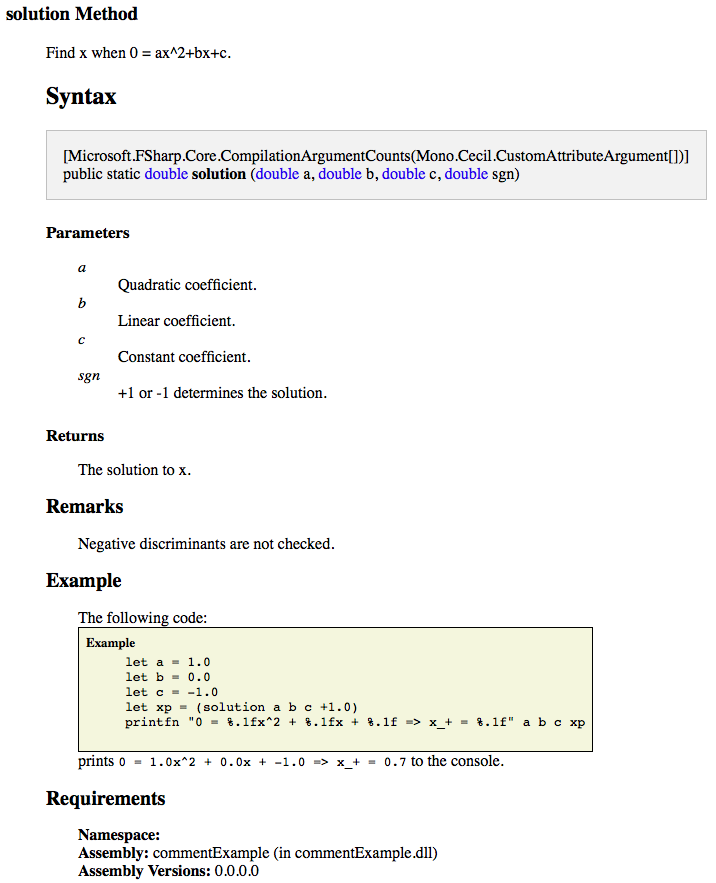
\includegraphics[width=\linewidth]{mdocOutput}
  \caption{Part of the HTML documentation as produce by \lstinline[language=console]{mdoc} and viewed in a browser.}
  \label{fig:htmlDocumentExample}
\end{figure}
A full description of how to use \lstinline[language=console]{mdoc} is found here\footnote{\url{http://www.mono-project.com/docs/tools+libraries/tools/monodoc/generating-documentation/}}.

%%% Local Variables:
%%% TeX-master: "fsharpNotes"
%%% End:
